


\tikzset{every picture/.style={line width=0.75pt}} %set default line width to 0.75pt        

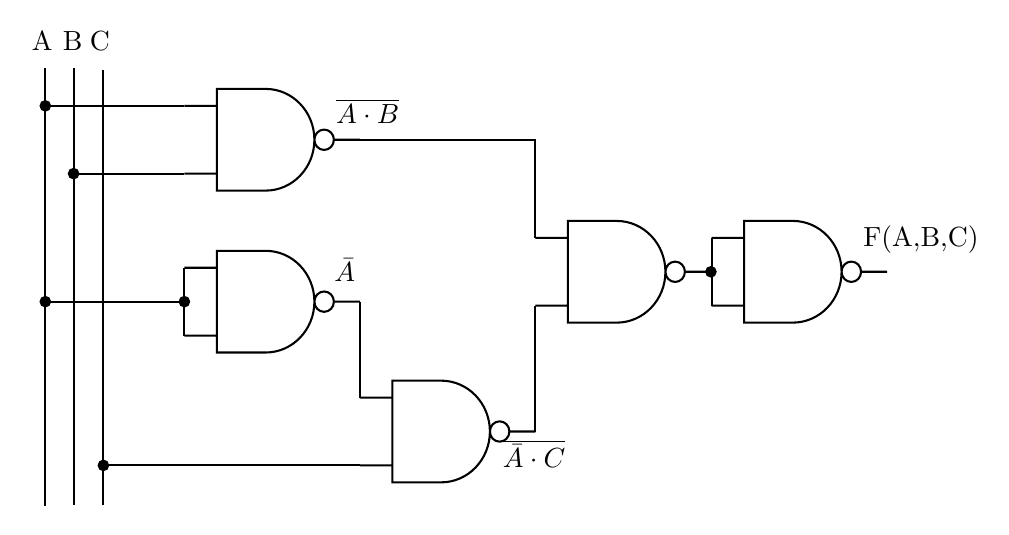
\begin{tikzpicture}[x=0.75pt,y=0.75pt,yscale=-1,xscale=1]
%uncomment if require: \path (0,349); %set diagram left start at 0, and has height of 349

%Shape: Nand Gate [id:dp7202246221683875] 
\draw   (110.66,111) -- (134.15,111) .. controls (147.11,111) and (157.64,121.98) .. (157.64,135.5) .. controls (157.64,149.02) and (147.11,160) .. (134.15,160) -- (110.66,160) -- (110.66,111) -- cycle (95,119.17) -- (110.66,119.17) (95,151.83) -- (110.66,151.83) (167.03,135.5) -- (179.56,135.5) (157.64,135.5) .. controls (157.64,132.79) and (159.74,130.6) .. (162.33,130.6) .. controls (164.93,130.6) and (167.03,132.79) .. (167.03,135.5) .. controls (167.03,138.21) and (164.93,140.4) .. (162.33,140.4) .. controls (159.74,140.4) and (157.64,138.21) .. (157.64,135.5) -- cycle ;
%Straight Lines [id:da5073209663512035] 
\draw    (42,101) -- (42,311.33) ;
%Straight Lines [id:da24811069484833514] 
\draw    (28,101) -- (28,311.73) ;
%Straight Lines [id:da08500169188449469] 
\draw    (56,102) -- (56,311.33) ;
%Shape: Nand Gate [id:dp726318471039981] 
\draw   (110.66,189) -- (134.15,189) .. controls (147.11,189) and (157.64,199.98) .. (157.64,213.5) .. controls (157.64,227.02) and (147.11,238) .. (134.15,238) -- (110.66,238) -- (110.66,189) -- cycle (95,197.17) -- (110.66,197.17) (95,229.83) -- (110.66,229.83) (167.03,213.5) -- (179.56,213.5) (157.64,213.5) .. controls (157.64,210.79) and (159.74,208.6) .. (162.33,208.6) .. controls (164.93,208.6) and (167.03,210.79) .. (167.03,213.5) .. controls (167.03,216.21) and (164.93,218.4) .. (162.33,218.4) .. controls (159.74,218.4) and (157.64,216.21) .. (157.64,213.5) -- cycle ;
%Straight Lines [id:da9397830971262995] 
\draw    (95,119.17) -- (28,119.17) ;
%Shape: Circle [id:dp42498686410328546] 
\draw  [fill={rgb, 255:red, 0; green, 0; blue, 0 }  ,fill opacity=1 ] (25.72,119.17) .. controls (25.72,117.91) and (26.74,116.89) .. (28,116.89) .. controls (29.26,116.89) and (30.28,117.91) .. (30.28,119.17) .. controls (30.28,120.43) and (29.26,121.45) .. (28,121.45) .. controls (26.74,121.45) and (25.72,120.43) .. (25.72,119.17) -- cycle ;
%Straight Lines [id:da36548282388341646] 
\draw    (95,151.83) -- (41.62,151.83) ;
%Shape: Circle [id:dp303857496497147] 
\draw  [fill={rgb, 255:red, 0; green, 0; blue, 0 }  ,fill opacity=1 ] (39.34,151.83) .. controls (39.34,150.57) and (40.36,149.55) .. (41.62,149.55) .. controls (42.88,149.55) and (43.9,150.57) .. (43.9,151.83) .. controls (43.9,153.09) and (42.88,154.11) .. (41.62,154.11) .. controls (40.36,154.11) and (39.34,153.09) .. (39.34,151.83) -- cycle ;
%Straight Lines [id:da7795697175741734] 
\draw    (95,197.17) -- (95,229.83) ;
%Straight Lines [id:da05123217043757178] 
\draw    (95,213.5) -- (28,213.5) ;
%Shape: Circle [id:dp9515785817279796] 
\draw  [fill={rgb, 255:red, 0; green, 0; blue, 0 }  ,fill opacity=1 ] (25.72,213.5) .. controls (25.72,212.24) and (26.74,211.22) .. (28,211.22) .. controls (29.26,211.22) and (30.28,212.24) .. (30.28,213.5) .. controls (30.28,214.76) and (29.26,215.78) .. (28,215.78) .. controls (26.74,215.78) and (25.72,214.76) .. (25.72,213.5) -- cycle ;
%Shape: Circle [id:dp17848478669324241] 
\draw  [fill={rgb, 255:red, 0; green, 0; blue, 0 }  ,fill opacity=1 ] (92.72,213.5) .. controls (92.72,212.24) and (93.74,211.22) .. (95,211.22) .. controls (96.26,211.22) and (97.28,212.24) .. (97.28,213.5) .. controls (97.28,214.76) and (96.26,215.78) .. (95,215.78) .. controls (93.74,215.78) and (92.72,214.76) .. (92.72,213.5) -- cycle ;
%Shape: Nand Gate [id:dp2947712634769619] 
\draw   (195.22,251.56) -- (218.71,251.56) .. controls (231.67,251.56) and (242.2,262.54) .. (242.2,276.06) .. controls (242.2,289.58) and (231.67,300.56) .. (218.71,300.56) -- (195.22,300.56) -- (195.22,251.56) -- cycle (179.56,259.73) -- (195.22,259.73) (179.56,292.39) -- (195.22,292.39) (251.59,276.06) -- (264.12,276.06) (242.2,276.06) .. controls (242.2,273.35) and (244.3,271.16) .. (246.89,271.16) .. controls (249.49,271.16) and (251.59,273.35) .. (251.59,276.06) .. controls (251.59,278.77) and (249.49,280.96) .. (246.89,280.96) .. controls (244.3,280.96) and (242.2,278.77) .. (242.2,276.06) -- cycle ;
%Straight Lines [id:da794649041002464] 
\draw    (179.56,213.5) -- (179.56,259.73) ;
%Straight Lines [id:da7045776504233234] 
\draw    (179.56,292.39) -- (55.98,292.39) ;
%Shape: Circle [id:dp9733182657274635] 
\draw  [fill={rgb, 255:red, 0; green, 0; blue, 0 }  ,fill opacity=1 ] (53.7,292.39) .. controls (53.7,291.13) and (54.72,290.11) .. (55.98,290.11) .. controls (57.24,290.11) and (58.26,291.13) .. (58.26,292.39) .. controls (58.26,293.65) and (57.24,294.67) .. (55.98,294.67) .. controls (54.72,294.67) and (53.7,293.65) .. (53.7,292.39) -- cycle ;
%Shape: Nand Gate [id:dp9831539452228355] 
\draw   (279.78,174.61) -- (303.27,174.61) .. controls (316.23,174.61) and (326.76,185.59) .. (326.76,199.11) .. controls (326.76,212.63) and (316.23,223.61) .. (303.27,223.61) -- (279.78,223.61) -- (279.78,174.61) -- cycle (264.12,182.78) -- (279.78,182.78) (264.12,215.44) -- (279.78,215.44) (336.15,199.11) -- (348.68,199.11) (326.76,199.11) .. controls (326.76,196.4) and (328.86,194.21) .. (331.45,194.21) .. controls (334.05,194.21) and (336.15,196.4) .. (336.15,199.11) .. controls (336.15,201.82) and (334.05,204.01) .. (331.45,204.01) .. controls (328.86,204.01) and (326.76,201.82) .. (326.76,199.11) -- cycle ;
%Straight Lines [id:da6270775361580909] 
\draw    (264.12,276.06) -- (264.12,215.44) ;
%Straight Lines [id:da4814129850836626] 
\draw    (179.56,135.5) -- (264.42,135.5) ;
%Straight Lines [id:da8924399219870336] 
\draw    (264.12,182.78) -- (264.12,135.44) ;
%Shape: Nand Gate [id:dp9179684426978327] 
\draw   (364.66,174.6) -- (388.15,174.6) .. controls (401.11,174.6) and (411.64,185.58) .. (411.64,199.1) .. controls (411.64,212.62) and (401.11,223.6) .. (388.15,223.6) -- (364.66,223.6) -- (364.66,174.6) -- cycle (349,182.77) -- (364.66,182.77) (349,215.43) -- (364.66,215.43) (421.03,199.1) -- (433.56,199.1) (411.64,199.1) .. controls (411.64,196.39) and (413.74,194.2) .. (416.33,194.2) .. controls (418.93,194.2) and (421.03,196.39) .. (421.03,199.1) .. controls (421.03,201.81) and (418.93,204) .. (416.33,204) .. controls (413.74,204) and (411.64,201.81) .. (411.64,199.1) -- cycle ;
%Straight Lines [id:da5368845385823731] 
\draw    (349,182.77) -- (349,215.43) ;
%Shape: Circle [id:dp6244252663534995] 
\draw  [fill={rgb, 255:red, 0; green, 0; blue, 0 }  ,fill opacity=1 ] (346.4,199.11) .. controls (346.4,197.85) and (347.42,196.83) .. (348.68,196.83) .. controls (349.94,196.83) and (350.96,197.85) .. (350.96,199.11) .. controls (350.96,200.37) and (349.94,201.39) .. (348.68,201.39) .. controls (347.42,201.39) and (346.4,200.37) .. (346.4,199.11) -- cycle ;

% Text Node
\draw (20,82) node [anchor=north west][inner sep=0.75pt]   [align=left] {A};
% Text Node
\draw (48,82) node [anchor=north west][inner sep=0.75pt]   [align=left] {C};
% Text Node
\draw (35,82) node [anchor=north west][inner sep=0.75pt]   [align=left] {B};
% Text Node
\draw (420.6,175.24) node [anchor=north west][inner sep=0.75pt]   [align=left] {F(A,B,C)};
% Text Node
\draw (165.8,191.24) node [anchor=north west][inner sep=0.75pt]   [align=left] {$\bar{A}$};
% Text Node
\draw (166.6,114.44) node [anchor=north west][inner sep=0.75pt]   [align=left] {$\overline{A\cdot B}$};
% Text Node
\draw (247,278.44) node [anchor=north west][inner sep=0.75pt]   [align=left] {$\overline{\bar{A}\cdot C}$};


\end{tikzpicture}